This section describes the various electronic components used in the project, as well as their interface to one another.  This section focuses on the hardware / electrical aspect of the components; one should refer to Section \ref{embeddedSoftwareAutomation} for details regarding the software implementation.  

\subsection{Hardware Components}
The following components were attached to an Atmel AT90 microcontroller either directly, or indirectly through a breadboard.  

\subsubsection{Atmel Microcontroller}
The Hovercraft project is centered around the AT90USB1287 processor from Atmel, mounted on a AT90USBKey which is shown in Figure \ref{fig:at90usbkey}.

\begin{minipage}{6.5in}
  \centering
    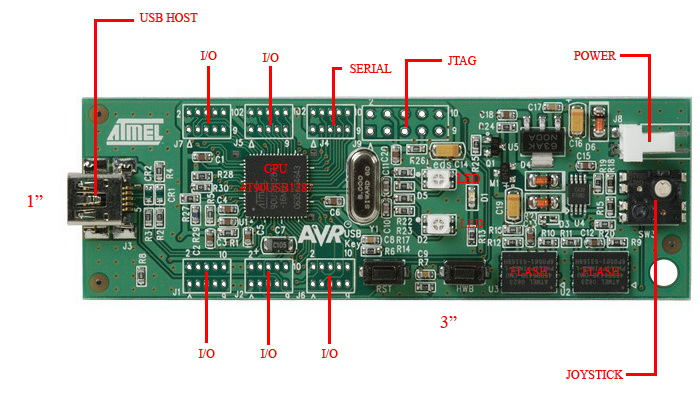
\includegraphics[width=110mm]{imageSources/at90usbkey.png}
 
  \captionof{figure}{Atmel AT90USBkey} 
  \label{fig:at90usbkey}
\end{minipage}

Some of the most notable features of this board include:
\begin{itemize}
\item USB Interface
\item 4+1-ways joystick
\item 2 Bi-Color LEDs
\item temperature sensor
\item serial dataflash memories
\item On-board RESET button 
\item On-board HWB button to force bootloader section execution at reset.
\item System clock: 8 MHz crystal
\end{itemize}

\subsubsection{Radio}
The radio used for hovercraft-basestation and hovercraft-hovercraft communication is the TRW-24G.  The datasheet for this component can be found here.  The radio operates at a frequency of 2.4 to 2.527 GHz and has a working voltage of 3 Volts (ranging from 1.8 to 3.6 Volts).  The radio can transit anywhere from 250 Kbps to 1000 Kbps (1Mbps).  Communication is segmented into 128 distinct channels which each occupy a 1 MHs chunk of spectrum. 

\begin{minipage}{6.5in}
  \begin{center}
    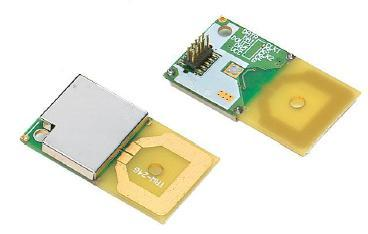
\includegraphics[width=110mm]{imageSources/radio.png}
  \end{center}
  \captionof{figure}{TRM-24G RF 2-way Radio} 
  \label{radioFig}
\end{minipage}

\subsubsection{Motors}
Several types of motors, as well as other supporting circuitry, are required to propel and maneuver the hovercraft.  

The DC Motor

The H-Bridge used is the L293D chip. This chip has the ability to run two H-bridges. 

  \begin{minipage}{6.5in}
        \centering
    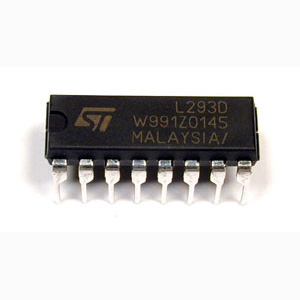
\includegraphics[width=110mm]{imageSources/hBridge.png}
  \captionof{figure}{L2930 H-Bridge} 
  \label{hBridge}
\end{minipage}



The L293D chip contains four input/output channels that can be used as two bridges. Each bridge (i.e. two channels) contains an enable connection required to operate the it. If the enable connection is given HIGH input, channel output is the same as channel input. If the enable is not connected or given LOW input, the channel output will be high impedance always. The L293D chip requires two connections at all times: a supply voltage (+5V) and ground (+0V). The chip also provides a second logic supply voltage if lower voltage operation is required.

The 74HC04 hex inverter chip is very simple. If the chip receives a HIGH signal, it will return a LOW signal, and visa versa. This hex inverter provides six input/output combinations. The inverter requires 5V of power and to be grounded.

\begin{minipage}{6.5in}
  \centering
    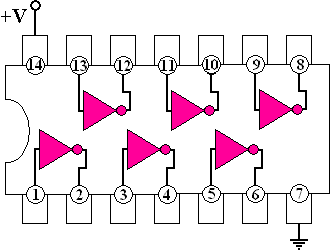
\includegraphics[width=110mm]{imageSources/hexInverter.png}
  
  \captionof{figure}{74HC04 Hex Inverter} 
  \label{hexInverter}
\end{minipage}

The servo used is the Hitec HS-55 who's datasheet can be found here. This is a very small servo that is controlled using pulse width control. It requires at least 4.8 volts of power, so it must be powered by the source, the AT90 only produces 3.3 volts.


  \begin{minipage}{6.5in}
    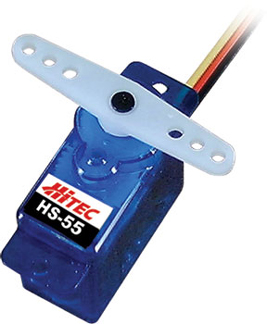
\includegraphics[width=90mm]{imageSources/servo.png}
  \centering
  \captionof{figure}{Hitec HS-55 Servo} 
  \label{servo}
\end{minipage}


\subsubsection{Joystick}
We used a traditional serial joystick. The joysticks port is a Male version of the above diagram. We then took a male connector and wired the ports that we wanted. X, Y ground and power. 


  \begin{minipage}{6.5in}
    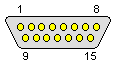
\includegraphics[width=90mm]{imageSources/joystick.png}
    \captionof{figure}{Joystick Pinout} 
  \label{joystick}
\end{minipage}


Table \ref{joystickPinout} describes the functions of each pin of the
joystick:

\begin{minipage}{6.5in}
\captionof{table}{The joystick pinout}
\begin{center}
\begin{tabular}{ c c c } 
  Pin Number & Signal Name & Description \\
  \hline
 1 & +5V & Power \\
 2 & Right Button 1 & Button 1 \\
 3 & X-Position 1 & Joystick 1 X-Coordinate \\
 4 & Signal GND & Ground \\
 5 & Signal GND & Ground \\
 6 & Y-Position 1 & Joystick 1 Y-Coordinate \\
 7 & Left Button 1 & Button 2 \\
 8 & +5V & Power \\
 9 & +5V & Power \\
 10 & Right Button 2 & Button 4/Joystick 2 Right button \\
 11 & X-Position 2 & Joystick 2 X-Coordinate \\
 12 & MIDI Out & MIDI Output \\
 13 & Y-Position 2 & Joystick 2 Y-Coordinate \\
 14 & Left Button 2 & Button 3/Joystick 2 Left button \\
 15 & MIDI In & MIDI Input \\
\end{tabular}
\label{joystickPinout}
\end{center}
\end{minipage}

\subsubsection{UART}
For testing purposes, when we wanted two UART readings, we used a windows machine and serial UART. For serial UART connections, the ADM33L chip is used to convert the signal. This chip is intended for use with transmitting and receiving devices. We use it for RS-232 transmission of data from the AT90 to a serial connection on a HyperTerminal running on the computer. This chip has an on board voltage converter to allow it to run from a single 5 volt power supply. 

  \begin{minipage}{6.5in}
    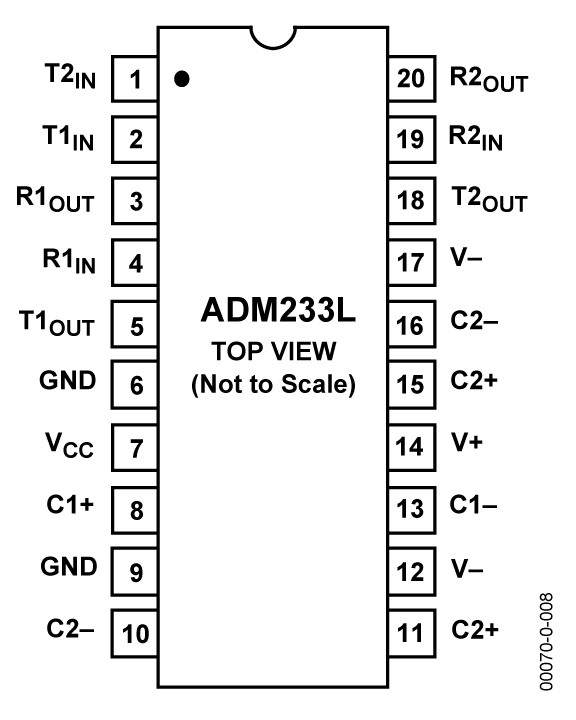
\includegraphics[width=90mm]{imageSources/serialUART.png}
  \centering
  \captionof{figure}{Serial UART Schematic} 
  \label{serialUART}
\end{minipage}


We are using USB to UART Bridge - FT232RL. This bridge is able to be connected directly to the board with out the use of an extra chip. This chip is powered using the 3.3 volts of power provided by the connection to the computer. 


  \begin{minipage}{6.5in}
    \centering
    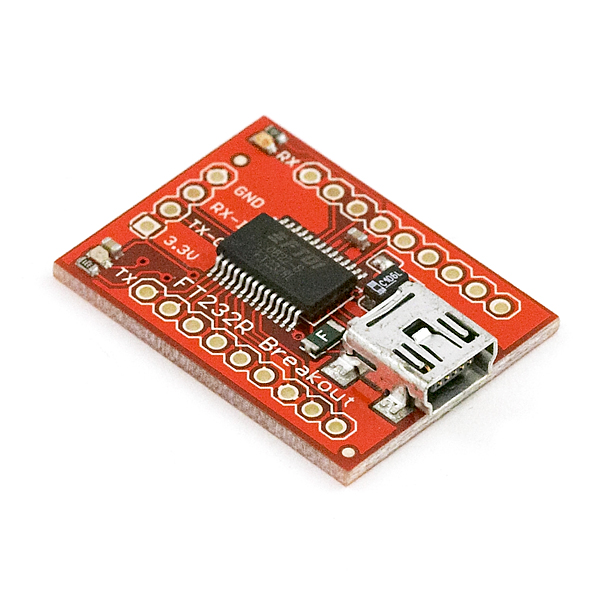
\includegraphics[width=90mm, height= 70mm]{imageSources/usbUART.png}
  \captionof{figure}{USB UART} 
  \label{usbUART}
\end{minipage}

\subsubsection{Sonar}
This sonar is capable of both long and short distance readings. It can tell if there is an object present from 0-254 inches, and gives distance information for objects 6-254 inches. This sonar has ground, VCC, enable and three different pins to read information(PWM, analog, digital). We chose to use the PWM.  When the enable pin is pulled high then the sonar will send out signals and listen.  The datasheet for the Max Sonar EZ1 can be found here.

  \begin{minipage}{6.5in}
    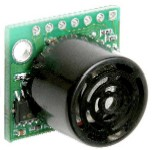
\includegraphics[width=70mm, height= 70mm]{imageSources/sonar.png}
  \centering
  \captionof{figure}{Max Sonar EZ1} 
  \label{sonar}
\end{minipage}

\subsection{Connections and Interface Design}
This section describes the connections among the various components, as well as other factors relating to the design of the electronic configurations used.  

\subsubsection{Power}
To power many of the components (Motors, Sonar, RS-232 Uart) we required more than the 3.3 volts of power than the USB provided. For this we needed to get power from the wall. Direct power from the wall reads between 9-12 Volts (our cords were supposed to produce 12, but they often had fluctuating readings).  This power needed to be minimized to a managable 5 volts.  The image below shows the setup to do this conversion.

  \begin{minipage}{6.5in}
    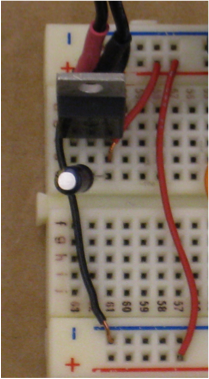
\includegraphics[scale=0.75]{imageSources/power12to5.png}
  \centering
  \captionof{figure}{Conversion from 12 to 5 volts} 
  \label{power12to5}
\end{minipage}

\subsubsection{Radio Connections}
\label{radioconn}


There is one radio present on each of the boards. The radio on the base station board sends the information regarding the position of the joystick and then prints the information it receives from the hover station.  The radio on the hovercraft sends information regarding the output of the motor and the sonar reading and receives information to change the position of the two motors.

All of the wires from the radio go to port E. The Radio ground pin must also be connected to the ground on the bread board. As modeled in the above diagram, the pin layout for the radios are as follows:

  \begin{minipage}{6.5in}
  \centering
    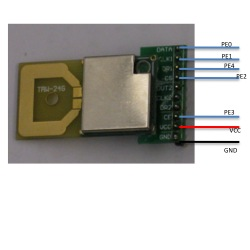
\includegraphics[width=90mm]{imageSources/radioConnect.png}
  
  \captionof{figure}{Radio Wiring Layout} 
  \label{radioConnect}
\end{minipage}

\subsubsection{Motor Connections}
An H-bridge is used to  control a motor that you want to spin in two different directions. Below is a diagram behind the theory of an H-Bridge taken from Wikipedia. An h-bridge is composed of a power source, four switches and a motor. The switches can all be in one of two positions, open or closed. There are only two different positions that the entire h-bridge can be in (shown in the diagram below). On the left, the lower left and upper right switches are open. this makes a circuit that goes through the motor from left to right, this will make the motor spin one way.  In the right diagram the other two switches are open, this makes the current flow through the motor from right to left, making the motor spin in the opposite direction.

  \begin{minipage}{6.5in}
    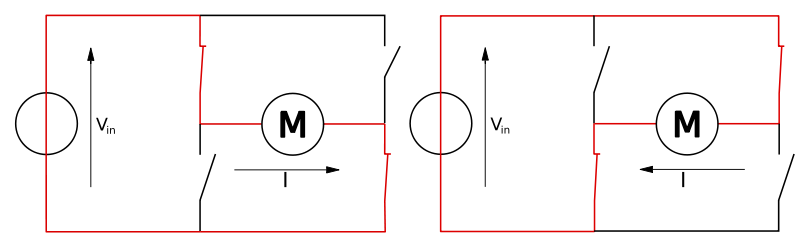
\includegraphics[width=90mm]{imageSources/hBridgeConnect1.png}
  \centering
  \captionof{figure}{Diagram of the H-bridge for a DC Motor} 
  \label{hBridgeConnect1}
\end{minipage}


  \begin{center}
    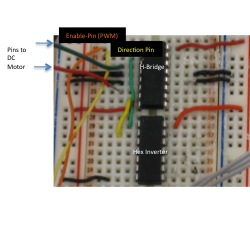
\includegraphics[width=90mm]{imageSources/hBridgeConnect2.png}
  \end{center}
  \captionof{figure}{Layout of the H-bridge} 
  \label{hBridgeConnect2}


In the above diagram, the orange enable pin is attached to OCR0A. This pin outputs the PWM signal needed to control the speed of the motor.  The yellow direction pin is connected to pin C1. This pin is either pulled HIGH or LOW which changes the position of the switches in the H-bridge.

\subsubsection{Joystick Connections}

For this project we are using an analog joystick. This means that  the joystick reads off many different readings to calculate its position. Details of how the conversion from analog to digital are outlined in the implementation section.

Pin 3, the x value, is wired to the first pin of PORT F (PINF1). The y value is connected to the second pin of PORT F (PINF2). Lastly, the second Y value is wired to the forth pin of PORT F (PINF4).

  \begin{minipage}{6.5in}
    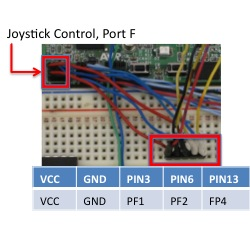
\includegraphics[width=90mm]{imageSources/joystickConnect.png}
  \centering
  \captionof{figure}{Joystick Connection: Pin Layout} 
  \label{joystickConnect}
\end{minipage}

\subsubsection{UART Connections}
The ADM233L connects to both the serial cable, and the AT90. 


  \begin{minipage}{6.5in}
    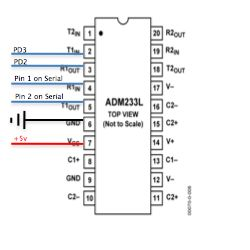
\includegraphics[width=90mm]{imageSources/uartConnect1.png}
  \centering
  \captionof{figure}{UART Pin Layout for ADM233L} 
  \label{uartConnect1}
\end{minipage}


  \begin{minipage}{6.5in}
    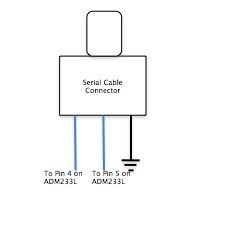
\includegraphics[width=90mm]{imageSources/uartConnect2.png}
  \centering
  \captionof{figure}{UART Pin Layout For Serial} 
  \label{uartConnect2}
\end{minipage}


  \begin{minipage}{6.5in}
    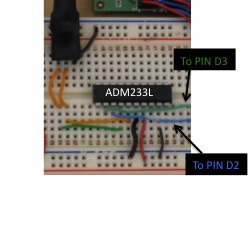
\includegraphics[width=90mm]{imageSources/uartConnect3.png}
  \centering
  \captionof{figure}{UART Wiring Layout} 
  \label{uartConnect3}
\end{minipage}

The above image is a picture of the UART layout of the board. In this picture, you can also see the layout for the power supply.

The USB UART is connected to the board on the same pins as the serial UART.  This chip has three output wires.  GND, TX-O, RX- I. This chip connects directly to the board. TX-O connects to PD2 and TX-I connects to PD3, the GND output connects directly to ground on the AT90.

\subsubsection{Servo Connections}
The servo motor requires 5 volts of power, to be connected to ground and a pwm signal to run. To generate the PWM signal a 16 bit timer must be enabled and the input wire on the servo must be connected to the proper output compare. For this component we used timer 1 and connected the servo to OC.1B which is located on PB6.

\subsubsection{Sonar Connections}
The sonar must be connected to two pins on the AT90 and to ground and power on the bread board. We decided to calculate the distance using PWM even though we could have used a few methods. (See sonar implementation for details on the conversion.)  For this the sonar needed to be attached to a pin on the board to be triggered when the input goes high. This pin also needs to be associated with a timer. We chose to use timer three for our sonar, and Input Capture Register (ICP3) to read the input which is located on port C7. The sonar will also only fire when the RX pin reads high. So we connected the RX pin to PC6 and then set that pin either high or low.

  \begin{minipage}{6.5in}
    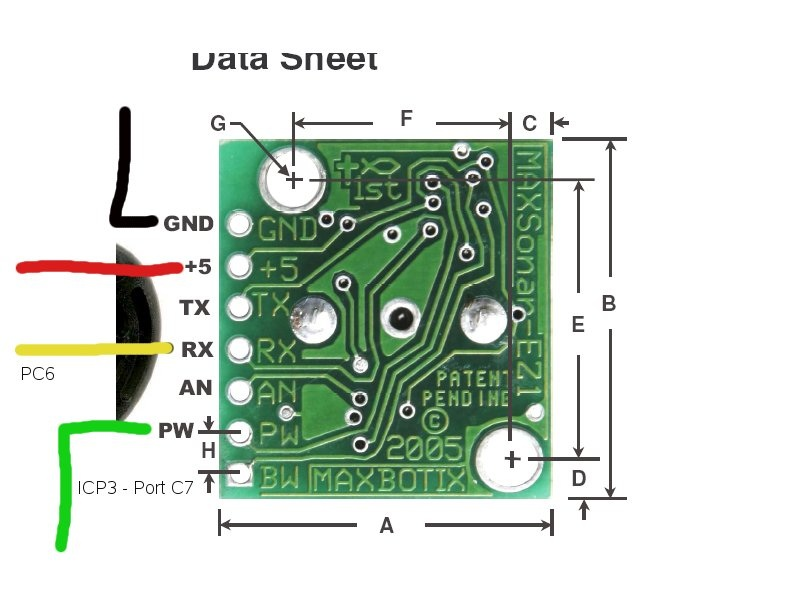
\includegraphics[width=90mm]{imageSources/sonarConnect.png}
  \centering
  \captionof{figure}{Sonar Wiring Layout} 
  \label{sonarConnect}
  \end{minipage}


